\documentclass[../../tc_tp6_main.tex]{subfiles}
\usepackage{tikzit}
\input{sample.tikzstyles}


\begin{document}
\chapter{PLL}

Un PLL es un circuito que permite generar una se\~nal de salida con la misma frecuencia que la se\~nal de entrada. Esta sincronizaci\'on se mantiene incluso con ruido en la entrada o con variaciones en la frecuencia de entrada dentro de cierto rango.

\section{Funcionamiento}

El PLL es un sistema realimentado en el cual se muestrea fase. Se dice que est\'a enganchado cuando la frecuencia de la entrada es la misma que la de la salida del VCO.

\begin{figure}[H]
	\centering 
	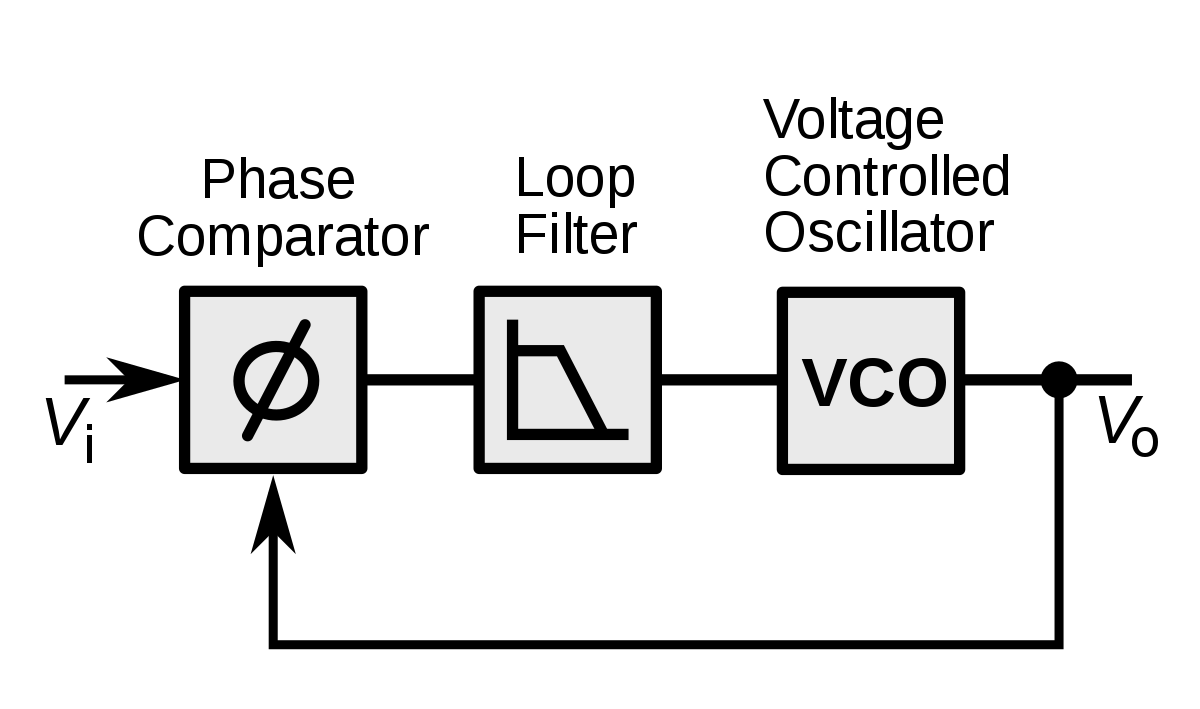
\includegraphics[width = 0.6\textwidth]{figures/pll_loop.png}
	\caption{Configuraci\'on b\'asica de un PLL}
	\label{fig:ej2_basic_pll}
\end{figure}

\subsection{Componentes}
\subsubsection{Comparador de fase}
El comparador de fase genera una se\~nal de salida ($v_E$, o se\~nal de error) cuyo valor medio es proporcional a la diferencia de fase entre dos se\~nales de entrada. Si $K_D$ es la ganancia del detector, se obtiene la expresi\'on del valor medio de la salida:
\begin{equation}
	valor \, medio \, v_E = K_D\cdot \Delta \phi
	\label{eq:ej2_salida_comparador}
\end{equation}

Cuando las dos entradas tienen la misma frecuencia constante, la salida del comparador tambi\'en es constante dado que $\Delta \phi$ no var\'ia. 

El integrado utilizado tiene dos tipos de comparadores de fase (tipo I y II), y se utiliz\'o el primero. \'Este es una compuerta XOR. Asumiendo que ambas entradas del comparador son se\~nales cuadradas entre 0 (low) y Vcc (high) con duty-cycle de 50\% y que las entradas tienen la misma frecuencia, la salida depende \'unicamente de la diferencia de fase seg\'un la ecuaci\'on \ref{eq:ej2_salida_comparador}. En la figura \ref{fig:ej2_xor_med} se muestra el funcionamiento del comparador para dos se\~nales de frecuencia constante.

\begin{figure}[H]
	\centering 
	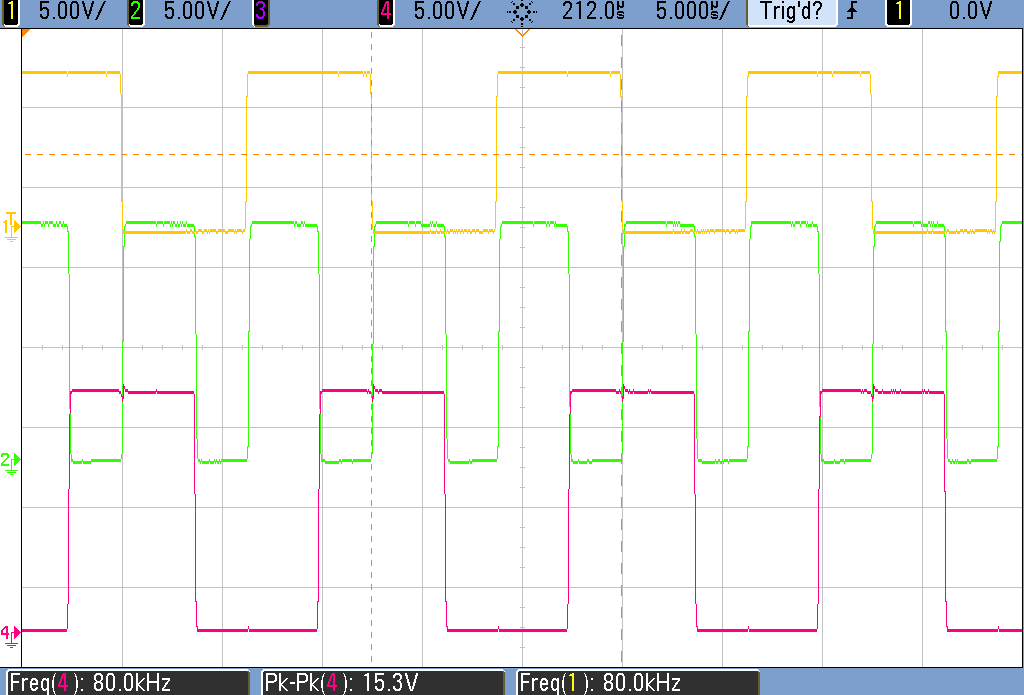
\includegraphics[width = 0.7\textwidth]{figures/xor.png}
	\caption{Medici\'on del comparador XOR (en amarillo y rosa las entradas y en verde la salida).}
	\label{fig:ej2_xor_med}
\end{figure}



\subsubsection{VCO}
El CD4046 tiene integrado un VCO, es decir, un oscilador controlado por tensi\'on continua con salida cuadrada. Se estudia en m\'as profundidad en el ejercicio 3.

\subsubsection{Filtro} \label{ssec:ej2_filtro}
La salida del comparador de fase utilizado no es una continua, sino una cuadrada con duty cycle variable. Para obtener el valor medio en continua para poder controlar el VCO, se utilizan dos filtros: RC y RRC.

\begin{figure}[H]	%gen vs demod
	\centering
	\begin{subfigure}[t]{0.35\textwidth}
		\centering
		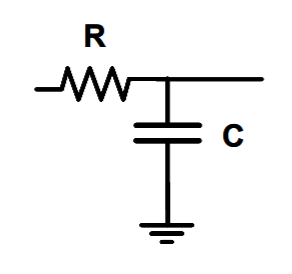
\includegraphics[width=\textwidth]{figures/rc.png}
		\caption{}
	\end{subfigure}%
	%\hfill%
	\begin{subfigure}[t]{0.35\textwidth}
		\centering
		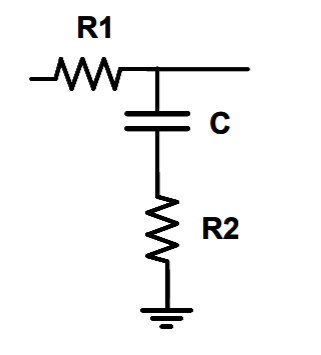
\includegraphics[width=\textwidth]{figures/rrc.png}
		\caption{}
	\end{subfigure}
	\caption{Esquem\'atico de los filtros del circuito}
	\label{fig:fm_rc_10k}
\end{figure}


Transferencia RC:
\[H(s) = \frac{1}{1+sRC}\]

Transferencia RRC:
\[H(s) = \frac{1+ sR_1C}{1+s(R_1+R_2)C}\]


\subsection{En enganche}

\begin{figure}
	\centering
	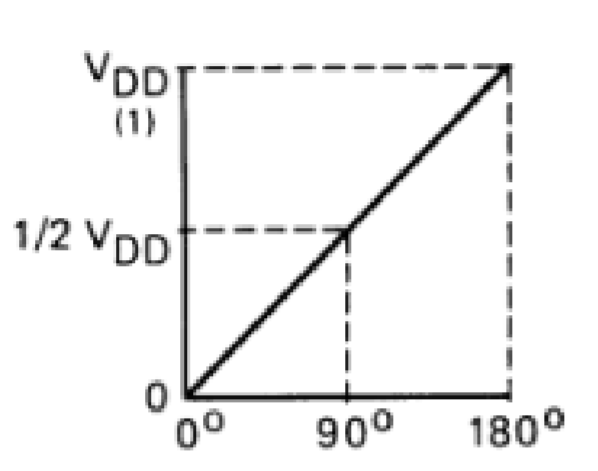
\includegraphics[width = 0.4\textwidth]{figures/fase_lineal.png}
	\caption{Relaci\'on entre el desfasaje y el valor medio de la tensi\'on de salida}
	\label{fase_lineal}
\end{figure}

Mientras mayor sea la frecuencia a la cual est\'e funcionado enganchado el PLL, mayor va a ser la tensi\'on necesaria a la entrada del VCO para poder generar dicha frecuencia. En consecuencia, mayor va a tener que ser el duty cycle de la salida del comparador. Se puede concluir, como muestra la figura \ref{fase_lineal}, que mientras mayor sea la frecuencia, mayor va a ser el desfasaje necesario para mantener el enganche. Se produce un desenganche cuando para mantener la frecuencia de la entrada el VCO necesita una tensi\'on que no puede ser alcanzada or el comparador ni siquiera con un desfasaje de 180$^\circ$

\subsection{Caracter\'isticas de los diferentes filtros}

\subsubsection{Respuesta al escal\'on de tensi\'on}
El filtro RRC tiene un tiempo de establecimiento menor que el RC. Como consecuecia, si se entra con una cuadrada de la misma frecuencia, la salida del RC va a estar m\'as acotada en amplitud que la del RRC. Esto es evidente en las respuestas al escal\'on de frecuencia (figura \ref{fig:escalon}).

\subsubsection{Respuesta al escal\'on de frecuencia, c\'alculo de Q y del tiempo de establecimiento}
Para la demodulaci\'on FM es de inter\'es la transferencia entre la frecuencia de la moduladora y la tensi\'on de entrada de VCO. En la figura \ref{fig:escalon} se muestra la tensi\'on en la entrada del VCO ante un escal\'on de frecuencia moduladora en la entrada (la portadora se mantiene fija en la $f_0$ correspondiente al filtro). En ambos casos se verific\'o que no se perdiera el enganche luego del salto.

Debido a bajos tiempos de establecimiento hacia la respuesta al escal\'on de tensi\'on, la respuesta al escal\'on de frecuencia es un banda de una ancho fijo y no una l\'inea. En todos los casos que se deban tomar valores de las mediciones, se toma el promedio lineal entre el ma\'ximo y el m\'inimo.

\[OS = \frac{V_{max}-V{final}}{V_{final}}\]
\[\zeta = \frac{-ln(OS)}{\sqrt{\pi ^2 + ln^2(OS)}}\]
\[Q = \frac{1}{2\zeta}\]


\begin{table}[H]
	\centering
	\begin{tabular}{|c|c|c|c|c|}
	\hline 
	 & OS & $\zeta$ & Q & T\\ 
	\hline 
	RC & 0.76 & 0.08 & 5.74 & 2.75 ms\\ 
	\hline 
	RRC & 0.45 & 0.24 & 2.05 & 100$\mu$ s \\ 
	\hline 
	\end{tabular} 
	\caption{\\OS: overshoot \\ $\zeta$: factor de amortiguamiento \\ Q: factor de calidad \\ T: tiempo de establecimiento al 2\%}
	\label{Q}
\end{table}

Se tendr\'ia m\'as precisi\'on en las mediciones anteriores si se hubiera tomado una medici\'on con m\'as cercan\'ia o si se hubieran posicionado convenientemente los cursores.

\begin{figure}[H]	%escalon frecuencia
	\centering
	\begin{subfigure}[t]{0.45\textwidth}
		\centering
		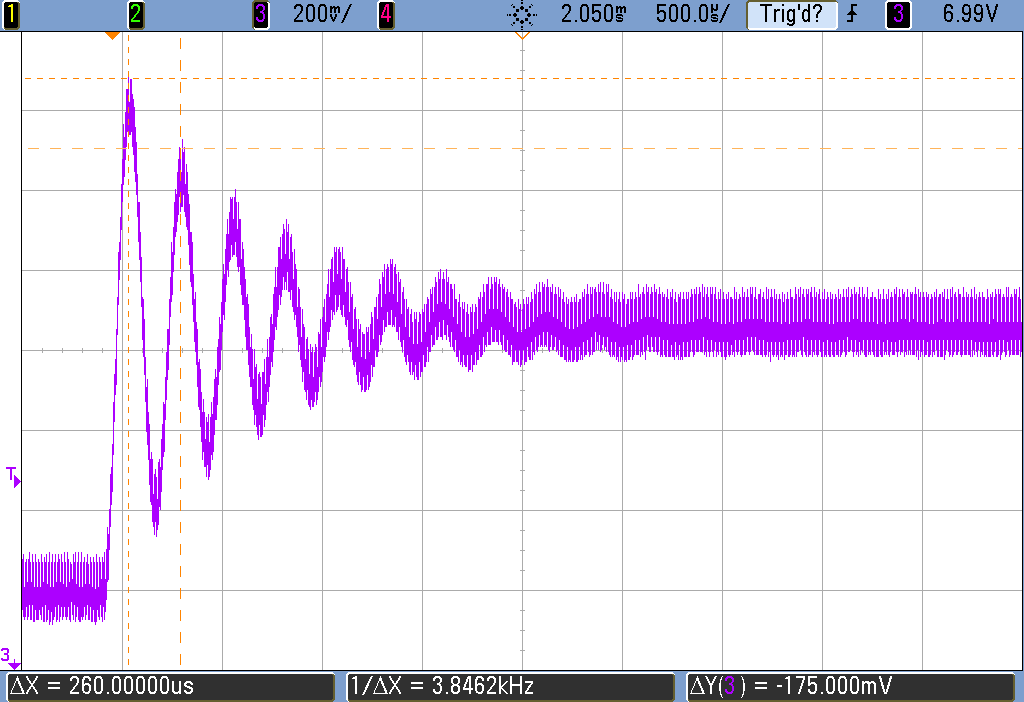
\includegraphics[width=\textwidth]{figures/escalon_rc.png}
		\caption{Filtro RC. Salto de frecuencia: 69KHz a 75KHz}
		\label{fig:escalon_RC}
	\end{subfigure}%
	\hfill%%
	\begin{subfigure}[t]{0.45\textwidth}
		\centering
		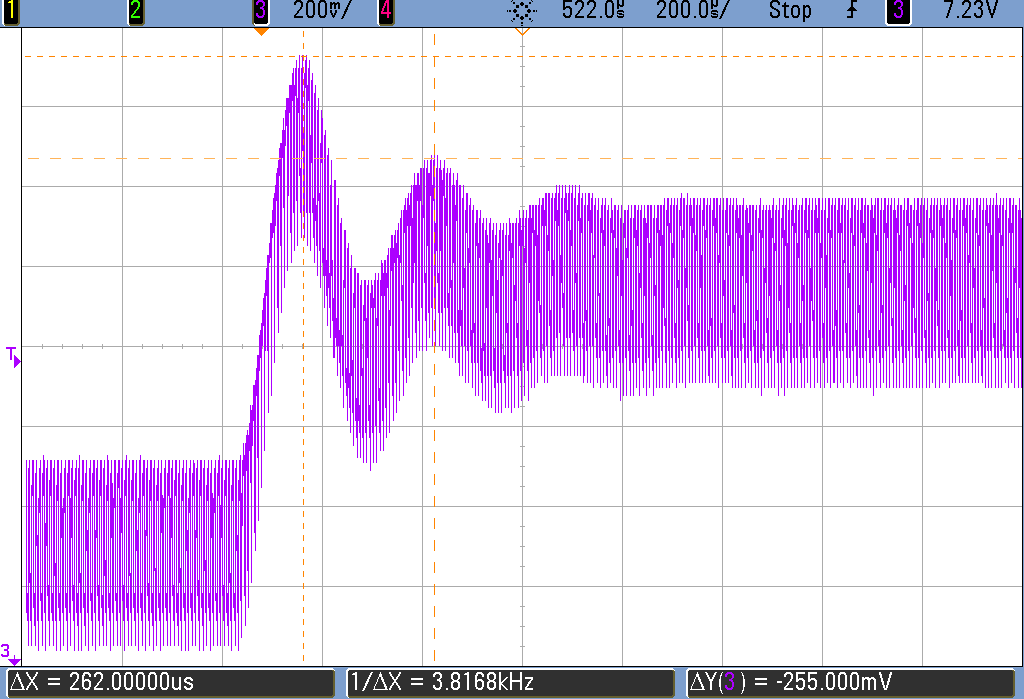
\includegraphics[width=\textwidth]{figures/escalon_rrc.png}
		\caption{Filtro RRC. Salto de frecuencia: 70KHz a 76KHz}
		\label{fig:escalon_RRC}
	\end{subfigure}
	\caption{Respuesta al escal\'on de la entrada del VCO con diferentes filtros de lazo. En ambos casos se verific\'o que la entrada y la salida estuvieran enganchadas antes y despues del salto. La portadora usada fue $f_0$.}
	\label{fig:escalon}
\end{figure}

Para ambos filtros se observa una respuesta subamortiguada con el mismo pseudoperiodo $f' = 3.8KHz$. El filtro RC tarda m\'as tiempo en establecerse que el RRC. Esto es favorable para ciertas aplicaciones, como por ejemplo para demodular se\~nales FM con saltos, como se observa en la figura \ref{fig:fm_rc_sq_500}. El RRC reproduce una copia mas cercana a la cuadrada debido a su menor tiempo de establecimiento. Sin embargo, tanto en el dominio del tiempo (comparando las dos se\~nales de la figura \ref{fig:fm_sq_500})  como en el dominio de la frecuencia (comparando las FFT de las figuras \ref{fig:fm_rrc_sq_500_demod} y \ref{fig:fm_rc_sq_500_gen}), se observa que hay considerables diferencias.


\begin{figure}[H]	%RC vs. RRC demod
	\centering
	\begin{subfigure}[t]{0.45\textwidth}
		\centering
		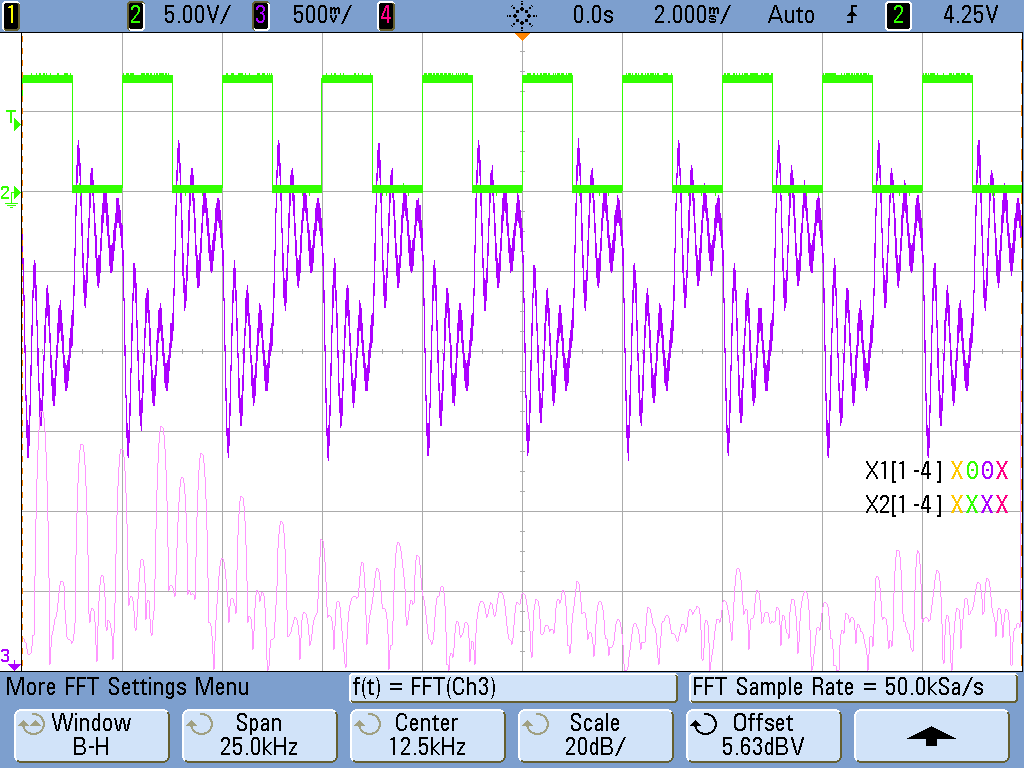
\includegraphics[width=\textwidth]{figures/fm_rc_sq_500_demod.png}
		\caption{Filtro RC}
		\label{fig:fm_rc_sq_500_demod_bis}
	\end{subfigure}%
	\hfill%%
	\begin{subfigure}[t]{0.45\textwidth}
		\centering
		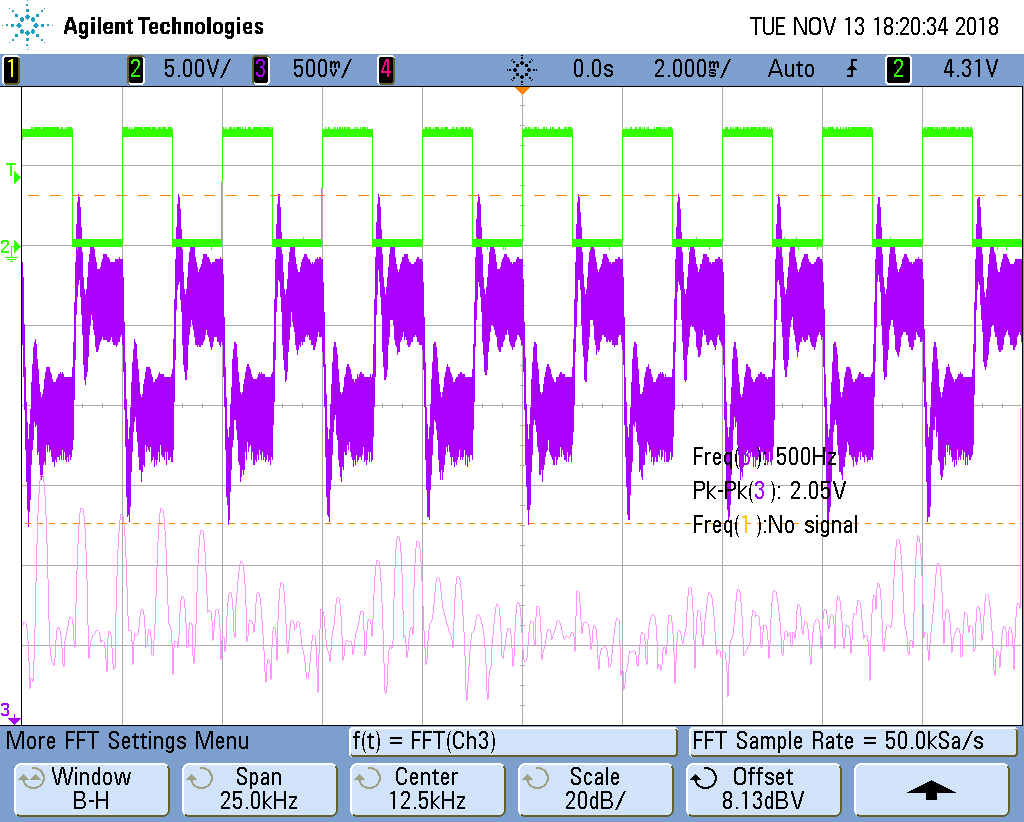
\includegraphics[width=\textwidth]{figures/fm_rrc_sq_500_demod.png}
		\caption{Filtro RRC}
		\label{fig:fm_rrc_sq_500_demod}
	\end{subfigure}
	\caption{Comparaci\'on de la demodulaci\'on FM de una se\~nal moduladora cuadrada de 500Hz con distintos filtros. En verde la se\~nal moduladora, en violeta la se\~nal demodulada.}
	\label{fig:fm_sq_500}
\end{figure}

\subsubsection{Rangos de enganche y de captura}

\begin{table}[H]
	\centering
	\begin{tabular}{|c|c|c|c|}
		\hline 
			& Rango captura & Rango enganche & $f_0$ \\ 
		\hline 
		sin filtro & 5KHz a 98KHz & 5KHz a 98KHz &  \\ 
		\hline 
		RC & 61KHz a 72KHz & 5KHz a 98KHz & 67KHz \\ 
		\hline 
		RRC & 56KHz a 79KHz & 5KHz a 98KHz & 71KHz \\ 
		\hline 
	\end{tabular}
	\caption{$f_0$ y rangos de captura y enganche medidos.}
	\label{tab:ej2_rangos}
\end{table}

El rango de enganche se mantiene constante en todos los filtros, pero la captura se facilita al usar el RRC por sobre el RC. \par 
En la figura \ref{fig:santi} se observa en verde la variaci\'on en el tiempo de la frecuencia de entrada desde 0 hasta 140KHz, y la variaci\'on en el valor medio del duty cycle. Cuando se encuentra en enganche, el duty aumenta o disminuye con la frecuencia. Esto sucede en los dos picos mayores (tanto ascendentes como descendentes). Se puede observar la diferencia entre el rango de enganche y de captura: si bien cuando aumenta la frecuencia el enganche se mantiene hasta los 98KHz, cuando se desengancha y disminuye, no se captura hasta los 72KHz aproximadamente. Lo mismo sucede si se disminuye la frecuencia hasta el desenganche.\par
Los picos secundarios observados suceden cuando el PLL se engancha a arm\'onicos de la frecuencia de entrada ya que se est\'a usando el comparador XOR.

\begin{figure}
	\centering
	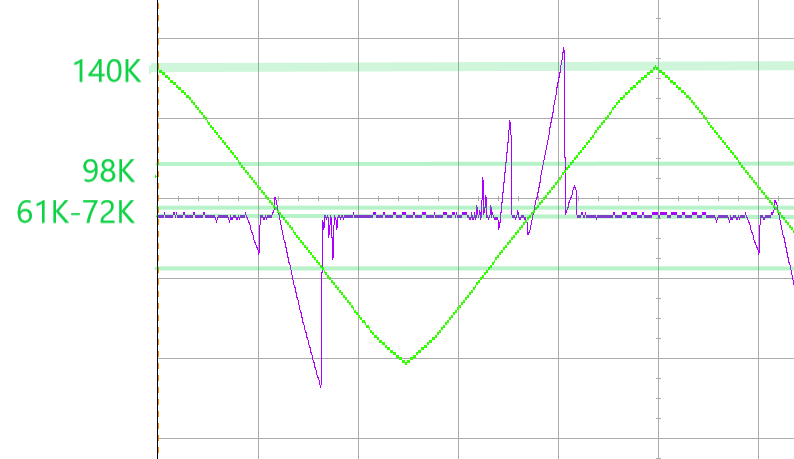
\includegraphics[width = 0.7\textwidth]{figures/gracias_santi.png}
	\caption{Medici\'on del rango de captura y de enganche del pll con el filtro RRC en el tiempo. En verde la frecuencia de la modulante, en violeta la entrada del VCO. Para mayor claridad en el gr\'afico, se us\'o el oscilocopio en modo high-resolution, lo que elimino el ripple de la entrada del VCO.}
	\label{fig:santi}
\end{figure}


\section{Aplicaciones}
\subsection{Uso como demodulador de FM}

Se utiliz\'o el circuito para demodular se\~nales FM. La portadora es siempre una frecuencia dentro del rango de enganche, mientras que la moduladora es una frecuencia menor a la portadora que puede estar fuera del rango de enganche, como por ejemplo en la figura \ref{fig:fm_rc_sq_500}.

Se observa en las figuras \ref{fig:fm_rc_10k} y \ref{fig:fm_rc_5k} que la demodulaci\'on mantiene la frecuencia aunque no puede mantener la forma de la onda.


\begin{figure}[H]	%gen vs demod
	\centering
	\begin{subfigure}[t]{0.45\textwidth}
		\centering
		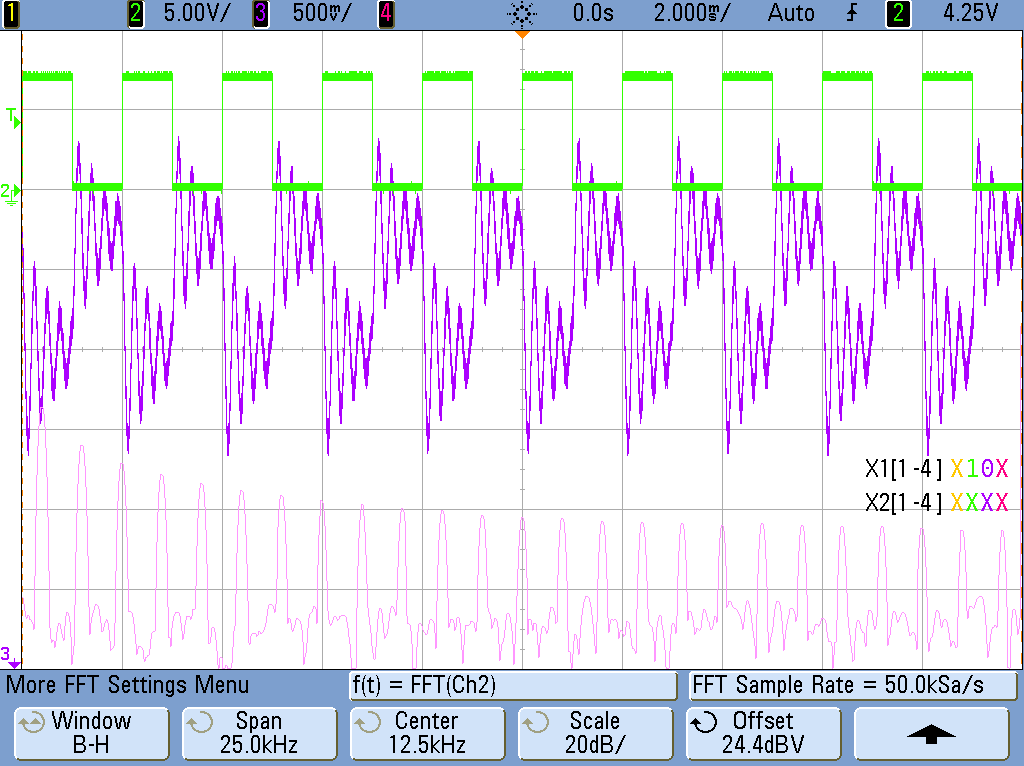
\includegraphics[width=\textwidth]{figures/fm_rc_sq_500_gen.png}
		\caption{FFT de la se\~nal del generador}
		\label{fig:fm_rc_sq_500_gen}
	\end{subfigure}%
	\hfill%%
	\begin{subfigure}[t]{0.45\textwidth}
		\centering
		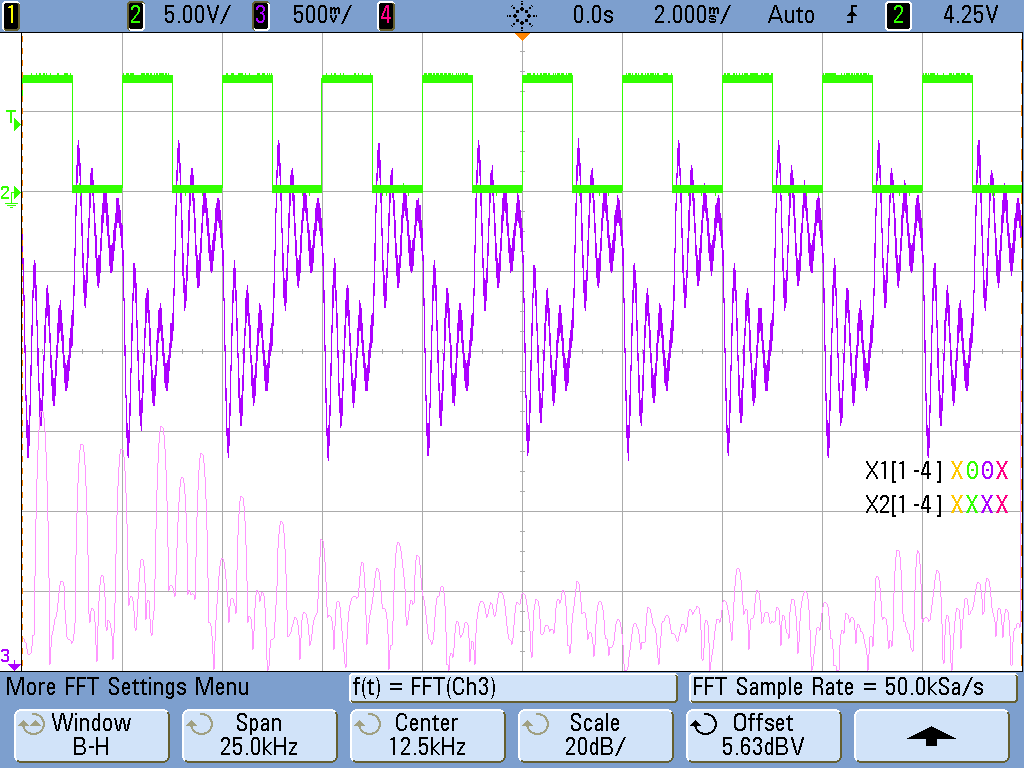
\includegraphics[width=\textwidth]{figures/fm_rc_sq_500_demod.png}
		\caption{FFT de la se\~nal demodulada}
		\label{fig:fm_rc_sq_500_demod}
	\end{subfigure}
	\caption{Comparaci\'on de las FFT de la demodulaci\'on y del generador de una moduladora de 500Hz. En verde la se\~nal moduladora, en violeta la se\~nal demodulada, y en rosa la FFT.}
	\label{fig:fm_rc_sq_500}
\end{figure}




\begin{figure}[H]	%gen vs demod
	\centering
	\begin{subfigure}[t]{0.45\textwidth}
		\centering
		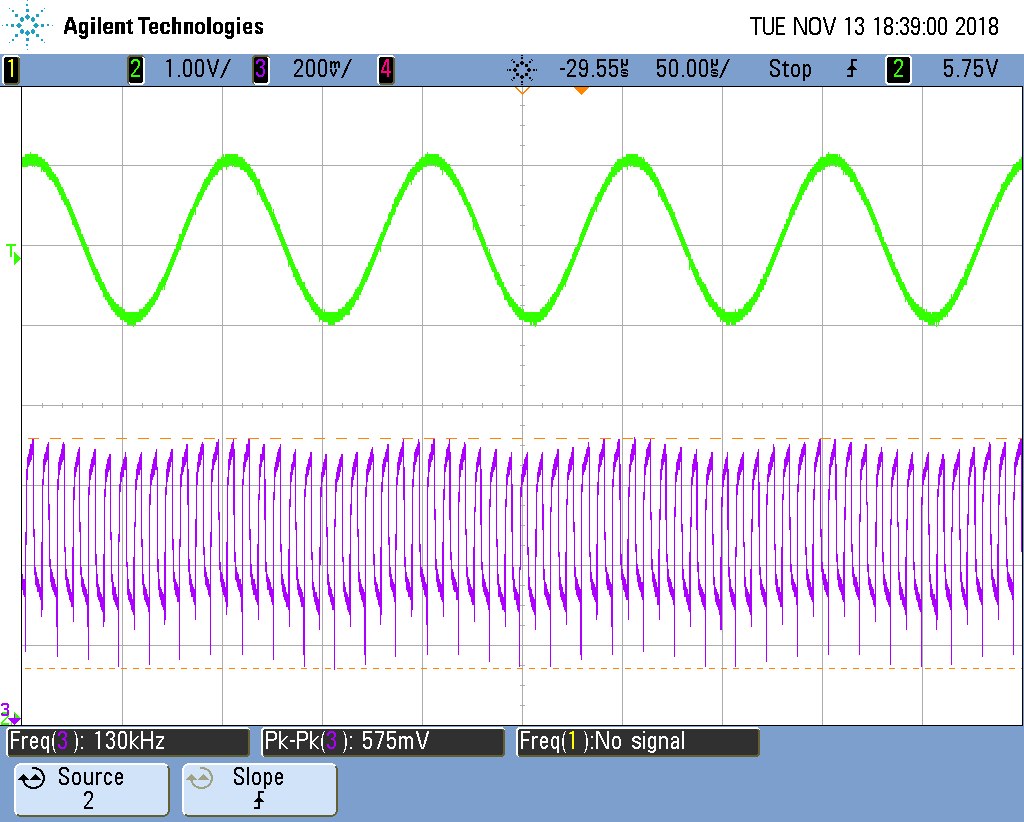
\includegraphics[width=\textwidth]{figures/scope_31.png}
		\caption{}
	\end{subfigure}%
	\hfill%%
	\begin{subfigure}[t]{0.45\textwidth}
		\centering
		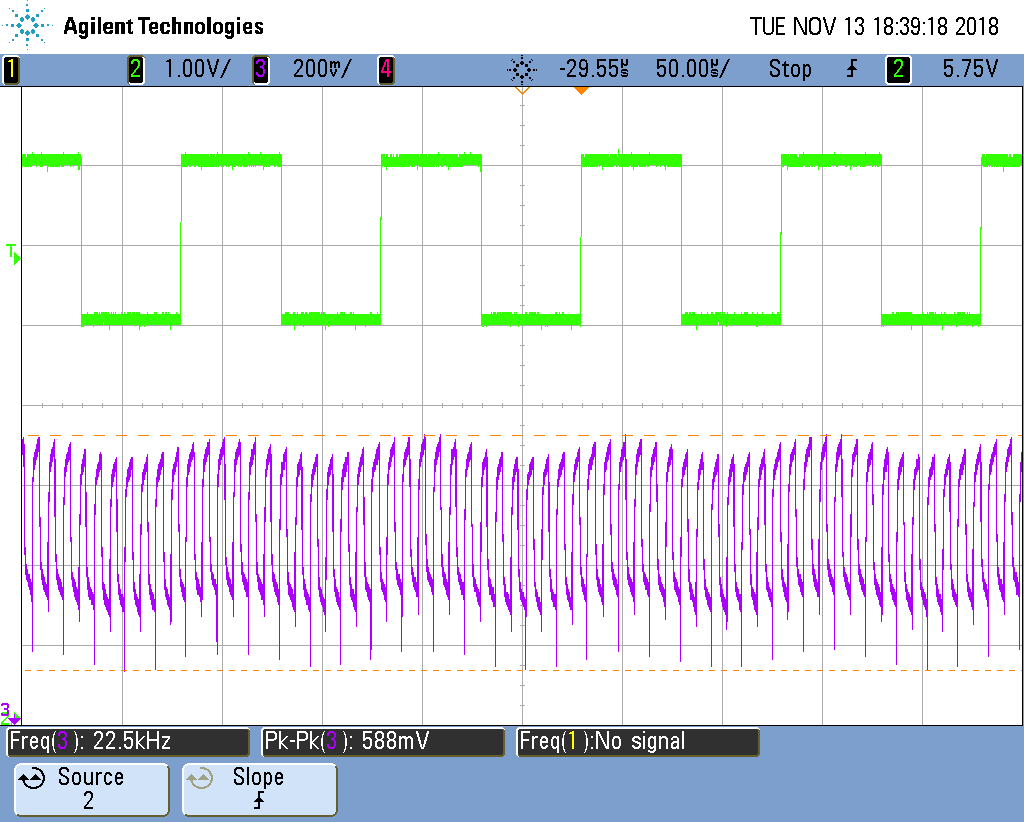
\includegraphics[width=\textwidth]{figures/scope_32.png}
		\caption{}
	\end{subfigure}
		\hfill%%
	\begin{subfigure}[t]{0.45\textwidth}
		\centering
		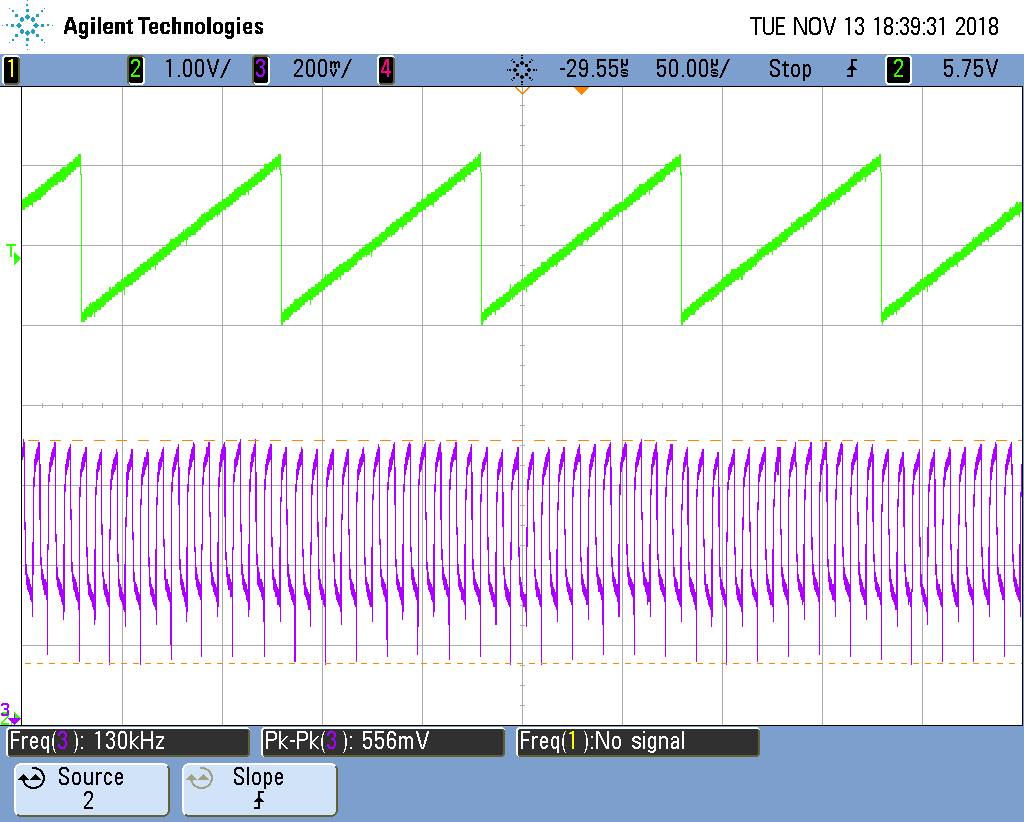
\includegraphics[width=\textwidth]{figures/scope_33.png}
		\caption{}
	\end{subfigure}
	\caption{Demodulaci\'on FM con el filtro RC a 10KHz. Moduladora en verda, demodulada en violeta.}
	\label{fig:fm_rc_10k}
\end{figure}

\begin{figure}[H]	%gen vs demod
	\centering
	\begin{subfigure}[t]{0.45\textwidth}
		\centering
		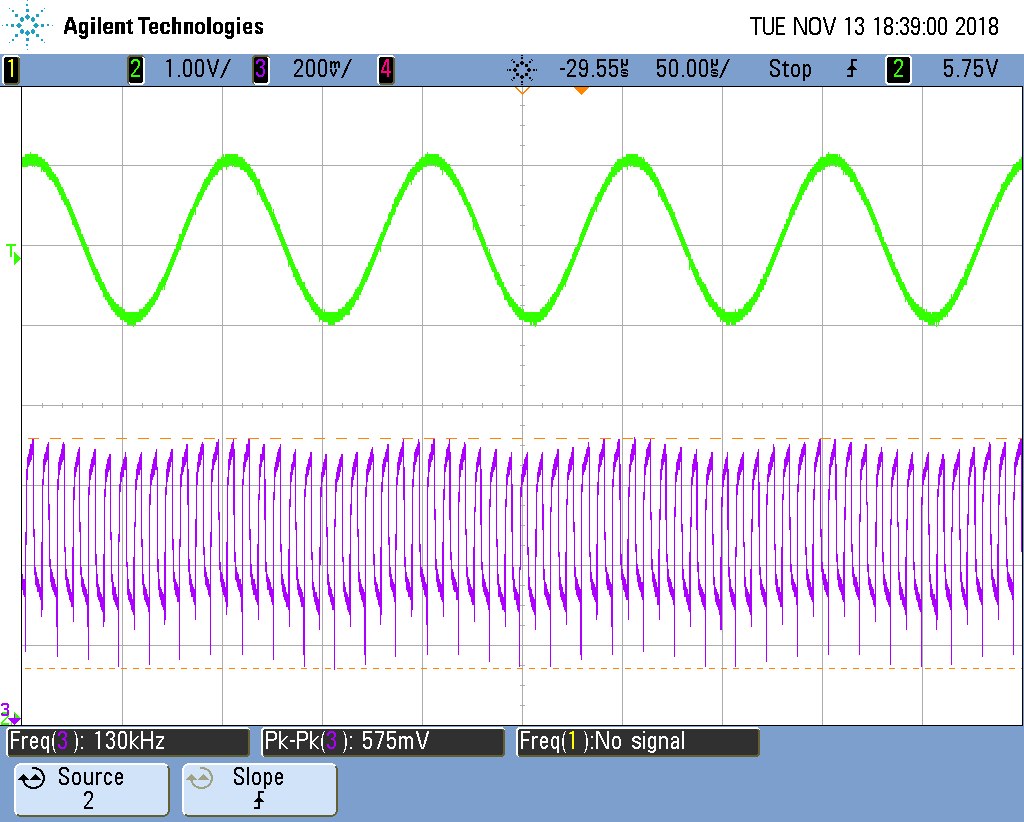
\includegraphics[width=\textwidth]{figures/scope_31.png}
		\caption{}
	\end{subfigure}%
	\hfill%%
	\begin{subfigure}[t]{0.45\textwidth}
		\centering
		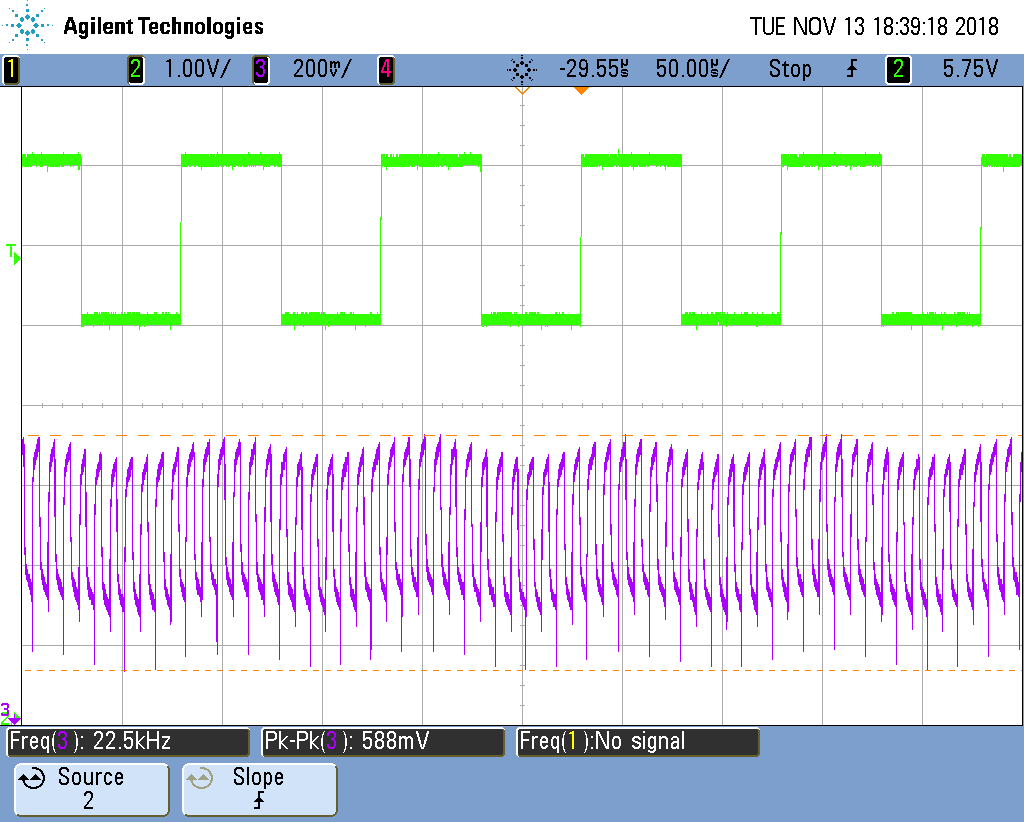
\includegraphics[width=\textwidth]{figures/scope_32.png}
		\caption{}
	\end{subfigure}
	\caption{Demodulaci\'on FM con el filtro RC a 10KHz. Moduladora en verde, demodulada en violeta.}
	\label{fig:fm_rc_10k}
\end{figure}


\begin{figure}
	\centering
	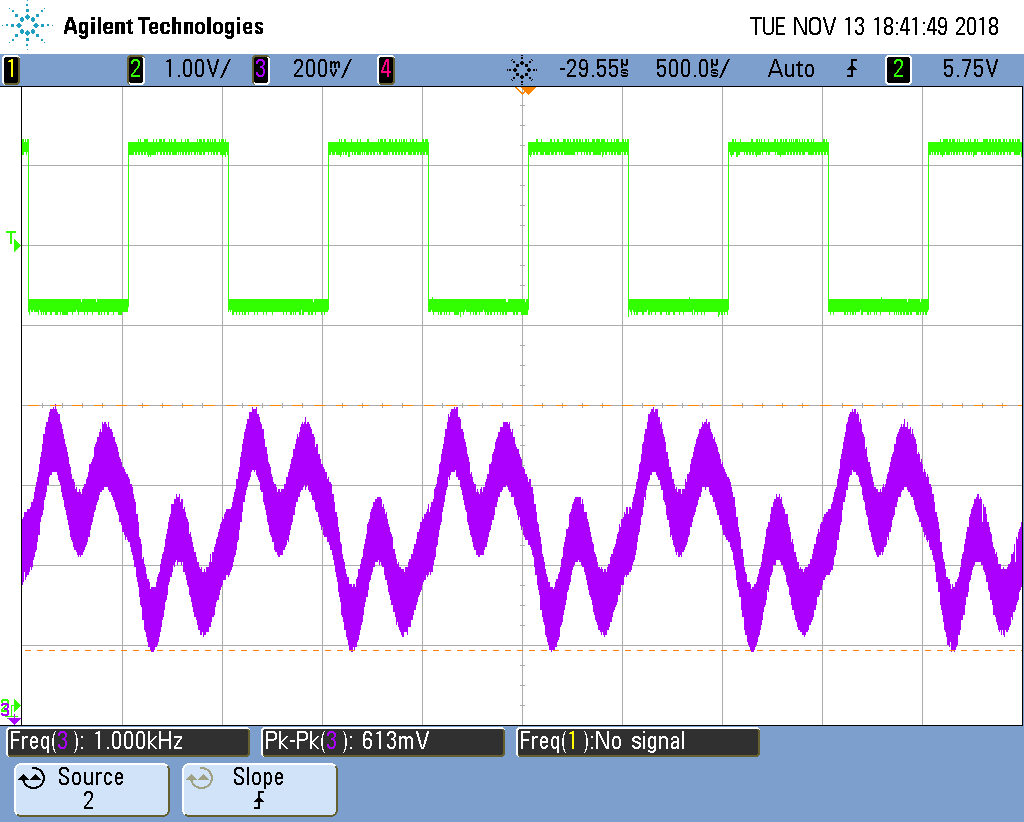
\includegraphics[width = 0.45\textwidth]{figures/scope_37.png}
	\caption{Demodulaci\'on FM con el filtro RC a 5KHz. Moduladora en verde, demodulada en violeta.}
	\label{fig:fm_rc_5k}
\end{figure}






\subsection{Uso como multiplicador de frecuencia}

Para estar en condici\'on de enganche, las frecuencias de entrada del comparador de fase deben estar a la misma frecuencia. Por lo tanto, al enganchar el PLL con un divisor de frecuencia en la posici\'on que indica la figura \ref{fig:multiplier_loop}, se asegura tener una frecuencia N veces m\'as grande que la de entrada en la salida del VCO.\par
Como el desenganche se da cuando para seguir la frecuencia de entrada el VCO necesita mas tensi\'on que la que el comparador con un duty cycle de 100\% puede darle, el rango de enganche con el multiplicador van a ser las frecuencias de entradas tales que la salida del VCO no superen el rango de enganche sin el divisor.


\begin{figure}[H]
	\centering
	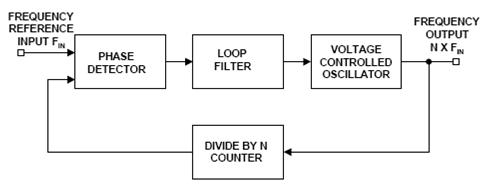
\includegraphics[width = \textwidth]{figures/multiplier_loop.jpg}
	\caption{Modificaci\'on del PLL para funcionar como multiplicador de frecuencias}
	\label{fig:multiplier_loop}
\end{figure}




\begin{figure}[H]	%multiplicador mediciones
	\centering
	\begin{subfigure}[t]{0.45\textwidth}
		\centering
		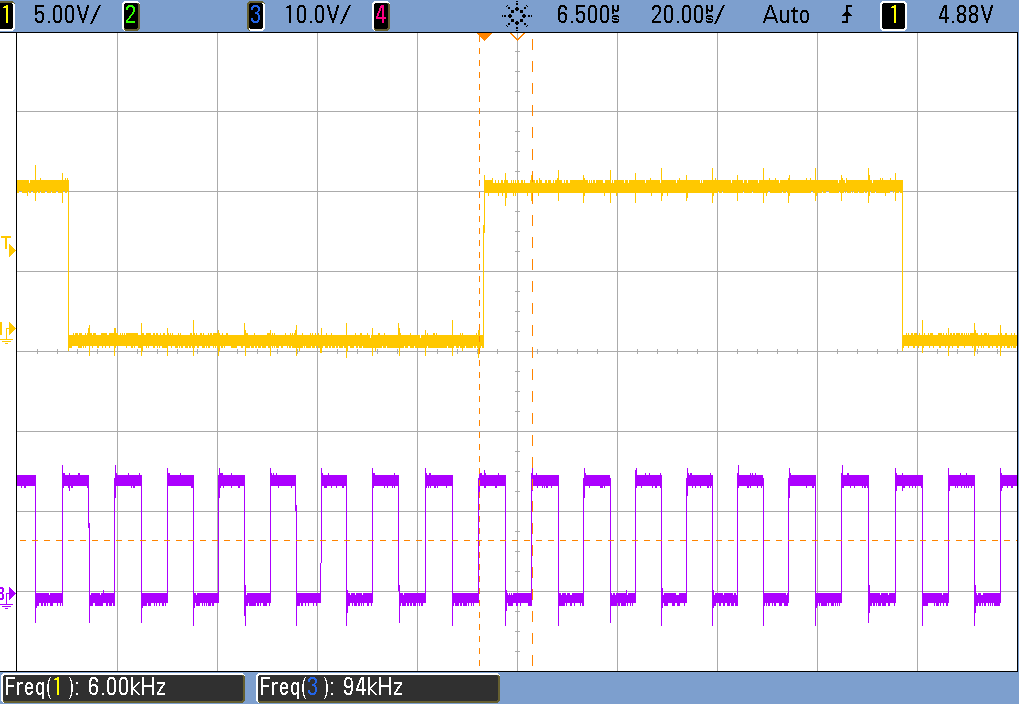
\includegraphics[width=\textwidth]{figures/mult_16_6k.png}
		\caption{A 6KHz}
		\label{fig:mult_16_6k}
	\end{subfigure}%
	\hfill%%
	\begin{subfigure}[t]{0.45\textwidth}
		\centering
		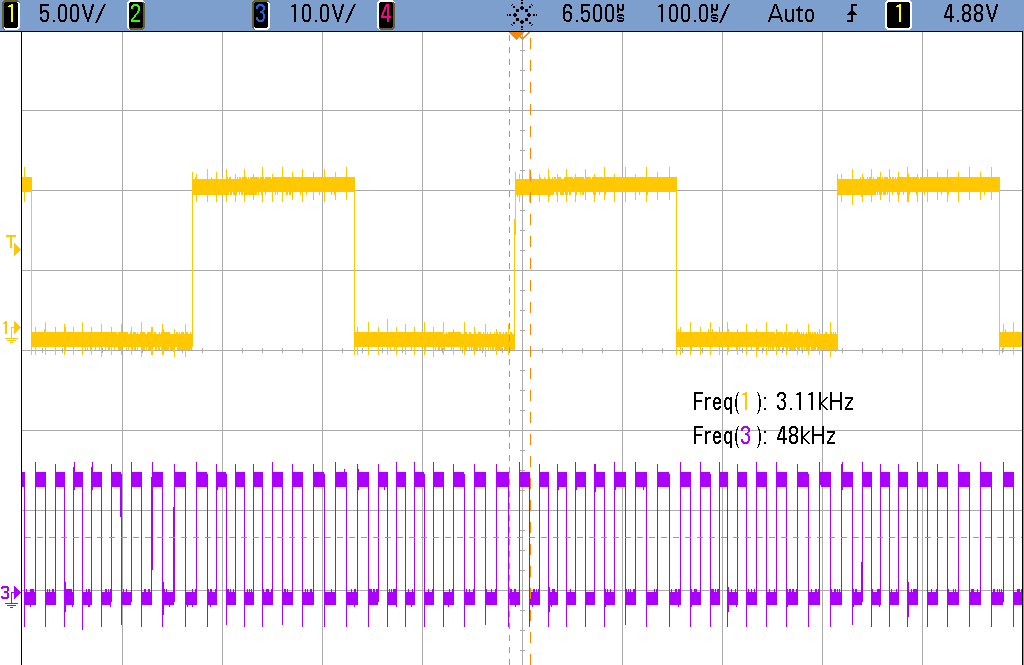
\includegraphics[width=\textwidth]{figures/mult_16_3k.png}
		\caption{A 3KHz. Notar que el enganche depende de la frecuencia de entrada al VCO (48KHz, perteneciente al rango de enganche) y no a la frecuecia de entrada (3KHz, no perteneciente al rango de enganche)}
		\label{fig:mult_16_3k}
	\end{subfigure}
	\caption{Multiplicador de frecuencia por 16. En amarillo la se\~nal de entrada y en violeta la entrada del VCO}
	\label{fig:mult_16}
\end{figure}



\end{document}
